\documentclass{beamer}
\usepackage{soul,color}
\usetheme{metropolis}           % Use metropolis theme
\title{Web Programming Lab}
\subtitle{Lesson 0 - Introduction to Linux \& Java}
%\date{\today}
\usepackage{lmodern}
\author{Giacomo Bergami}
\institute{University of Bologna}
\begin{document}
  \maketitle
  
    \begin{frame}{Introduction}
    Personal Information:
    \begin{itemize}
    	\item My web address: \url{http://jackbergus.github.io/teaching/LPI17/}
    	\item My e-mail: \href{mailto:giacomo.bergami2@unibo.it}{giacomo.bergami2@unibo.it}
    \end{itemize}
    
    Exercise 0:
  	\begin{itemize}
  		\item For these lab sessions, we're going to use the  \texttt{/public/lpi07/slot0$k$} folder.
  		\item Create a folder called \texttt{surname.name}
  		\item Copy the script \texttt{creation.sh} your freshly created directory.
  		\item Run it.
  	\end{itemize}
  \end{frame}
  
  \begin{frame}{Exercises 1-6}
    \begin{itemize}
    	\item Open the terminal. 
    	\item The terminal starts to work in your home directory, $\sim$, that is \texttt{/home/students/name.surname$k$/}
    	\item \texttt{\color{green} pwd} returns your current directory
    	\item \texttt{\color{green}cd \textbf{\color{red}folder}} stands for ``change directory'', it allows you to move throughout the file system.
    	\item \texttt{\color{green}mkdir \textbf{\color{red}folder}} allows to create a new folder.
    	\item \texttt{\color{green}touch \textbf{\color{red}file}} allows to either create a new file, or to update its ``timestamp''
    \end{itemize}
  \end{frame}

\begin{frame}{Exercises 1}
\begin{figure}
	\centering
	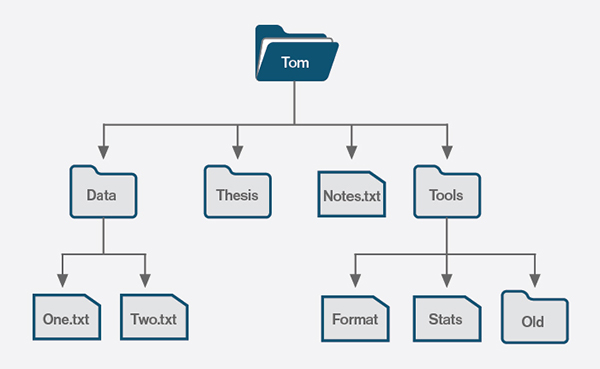
\includegraphics[width=0.7\linewidth]{00shell}
	\caption{An example of your home folder (\texttt{Tom})}
	\label{fig:00shell}
\end{figure}
\textbf{Move to folder Data:} \pause \texttt{cd Data}
\underline{You cannot \texttt{cd} a file (\texttt{cd Notes.txt} is not allowed)}
\end{frame}

\begin{frame}{Exercises 2}
	\begin{figure}
		\centering
		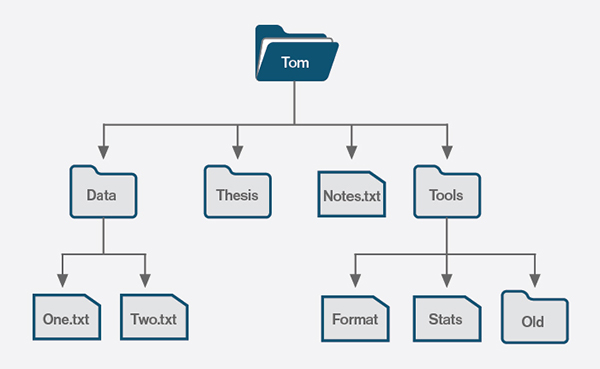
\includegraphics[width=0.7\linewidth]{00shell}
		\caption{An example of your home folder (\texttt{Tom})}
		\label{fig:00shell}
	\end{figure}
	\textbf{What is the result of pwd?} \pause \texttt{/home/students/Tom/Data}
\end{frame}

\begin{frame}{Exercises 3}
	\begin{figure}
		\centering
		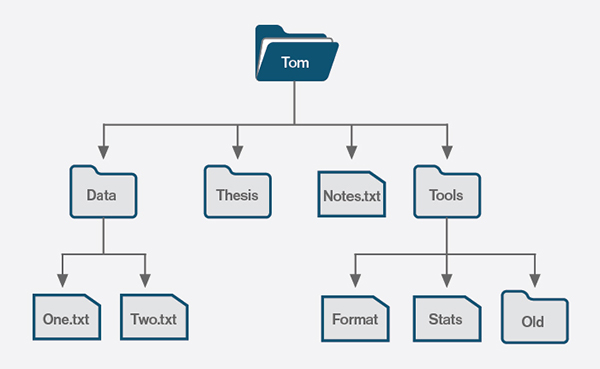
\includegraphics[width=0.7\linewidth]{00shell}
		\caption{An example of your home folder (\texttt{Tom})}
		\label{fig:00shell}
	\end{figure}
	\textbf{Create a new file Three.txt:} \pause \texttt{touch Three.txt}
\end{frame}

\begin{frame}{Exercises 4}
	\begin{figure}
		\centering
		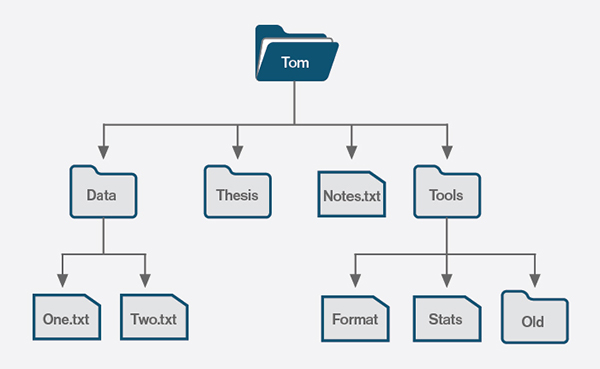
\includegraphics[width=0.7\linewidth]{00shell}
		\caption{An example of your home folder (\texttt{Tom})}
		\label{fig:00shell}
	\end{figure}
	\textbf{Move back to the parent folder:} \pause \texttt{cd ..}
	
	Two dots \texttt{..} always represents the parent folder.
\end{frame}

\begin{frame}{Exercises 5}
	\begin{figure}
		\centering
		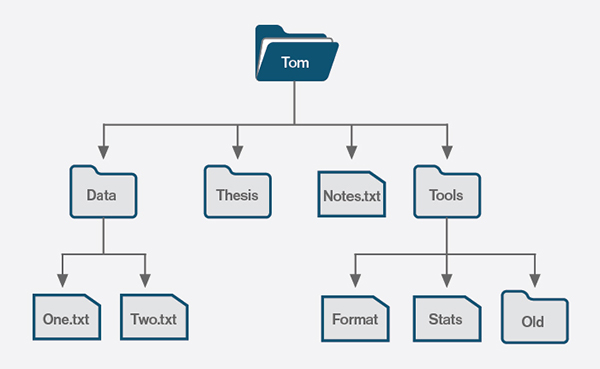
\includegraphics[width=0.7\linewidth]{00shell}
		\caption{An example of your home folder (\texttt{Tom})}
		\label{fig:00shell}
	\end{figure}
	\textbf{Move to folder Old} \pause \texttt{cd Tools/Old}
	
	One backslash \texttt{/} represents the path separator. A path connects distinct folders with a ``father-of'' relationship.
	\texttt{..} can be also used within a path.
\end{frame}

\begin{frame}{Exercises 6}
	\begin{figure}
		\centering
		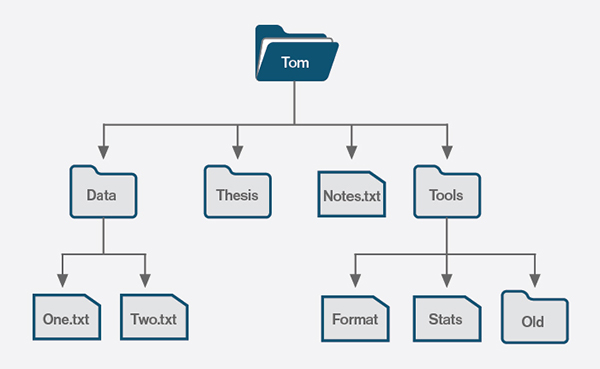
\includegraphics[width=0.7\linewidth]{00shell}
		\caption{An example of your home folder (\texttt{Tom})}
		\label{fig:00shell}
	\end{figure}
	\textbf{Move to folder Format} \pause \texttt{cd ../Format}
\end{frame}

\begin{frame}{Tip}
	When you want to open your editor and start with a new file, you can directly type \texttt{youreditor newfile.ext}. Those are some examples:
	\begin{itemize}
		\item \texttt{gedit HelloWorld.java}
		\item \texttt{jedit server.c}
		\item \texttt{geany MapReduce.cpp}
	\end{itemize}
 \textbf{NOTE:} if you want to still use the terminal after launching the command, put \texttt{\&} after launching the command.
\end{frame}

\begin{frame}{Exercise 7}
	\begin{itemize}
		\item The command to remove used to remove elements within the filesystem is \texttt{rm}
		\item The command  \texttt{\color{green} rm \textbf{\color{blue} file}} removes only files.
		\item In order to remove a folder, you have to remove all the files and folders contaned inside it. Hence, you have to type  \begin{center}
			\texttt{\color{green} rm -r \textbf{\color{blue} folder}}
		\end{center} where \texttt{-r} stands for ``recursively''
		\item \textbf{Exercise}: create a file (and a folder) and then remove it.
	\end{itemize}
\end{frame}


\begin{frame}{Programming languages}
	\begin{itemize}
		\item A programming language ($\mathcal{L}$) is a human readable language, that provides an abstraction from low level machine operations.
		\item All the programs $p$ written in a given language $\mathcal{L}$ cannot be read directly by your computer. Such programs have to be translated into a machine readable form.
		\item The compiler $\mathcal{C}$ is a program (function) converting a program $p$ from a language $\mathcal{L}$ into a (machine readable) language $\mathcal{M}$. $\mathcal{C}\colon \mathcal{L}\to \mathcal{M}$.
		\item An interpreter $\mathcal{I}_{\mathcal{M}}^{\mathcal{L}}$ for a lanugage $\mathcal{L}$ is a program written in the machine language $\mathcal{M}$ that runs a program $p$ written for a language $\mathcal{L}$.
	\end{itemize}
\begin{center}
\textit{Some help}: \url{https://drive.google.com/open?id=0B5EQQQtU0zzpWlp3V0RjNXBnNEk}
\end{center}
\end{frame}

\begin{frame}{Programming language: C++}
	\begin{itemize}
		\item The C compiler $\texttt{gcc}$ directly compiles the program written in C into a machine readable language $\mathcal{M}$. Such compiler is a function $\texttt{gcc}\colon C\to \mathcal{M}$.
		\item The program $\texttt{gcc}(p)$ requires no interpreter.
	\end{itemize}
\end{frame}

\begin{frame}{Programming language: Java (1)}
	\begin{itemize}
		\item The Java compiler $\texttt{javac}$ compiles the program written in Java into an intermediate bytecode $\mathcal{JVM}$. Such compiler is a function $\texttt{javac}\colon Java\to \mathcal{JVM}$.
		\item The programs compiled for the $\mathcal{JVM}$ cannot be directly read by the machine $\mathcal{M}$, and hence it requires an interpreter $\mathcal{I}_{\mathcal{M}}^{\mathcal{JVM}}$, called \textbf{Java Virtual Machine} (\texttt{java}).
		\item The compiled program $\texttt{javacc}(p)$ has to be run with such interpreter:
		\[\mathcal{I}_{\mathcal{M}}^{\mathcal{JVM}}(\texttt{javac}(p))\]
	\end{itemize}
\end{frame}

\begin{frame}{Programming language: Java (1)}
	\begin{itemize}
		\item The Java compiler $\texttt{javac}$ compiles the program written in Java into an intermediate bytecode $\mathcal{JVM}$. Such compiler is a function $\texttt{javac}\colon Java\to \mathcal{JVM}$.
		\item The programs compiled for the $\mathcal{JVM}$ cannot be directly read by the machine $\mathcal{M}$, and hence it requires an interpreter $\mathcal{I}_{\mathcal{M}}^{\mathcal{JVM}}$, called \textbf{Java Virtual Machine} (\texttt{java}).
		\item The compiled program $\texttt{javacc}(p)$ has to be run with such interpreter:
		\[\mathcal{I}_{\mathcal{M}}^{\mathcal{JVM}}(\texttt{javac}(p))\]
	\end{itemize}
\end{frame}

\begin{frame}{Programming language: Java (1)}
	\begin{itemize}
		\item The Java compiler $\texttt{javac}$ has to be invoked on a given source code file:
		\begin{center}
			\texttt{javac HelloWorld.java}
		\end{center}
		\item The Java interpreter $\texttt{java}$ tries to find the generated class file:
		\begin{center}
			\texttt{java HelloWorld}
		\end{center}
		\item \textbf{NOTE:} even though \texttt{javac HelloWorld.java} generates a file named \texttt{HelloWorld.class}, you shall not invoce \texttt{java HelloWorld.class}.
	\end{itemize}
\end{frame}


\begin{frame}{Coding Exercises}
	\begin{enumerate}
		\item Create a program that prints ``Hello World''.
		\begin{itemize}
			\item The class is the minimal functional unit of an \texttt{Object Oriented} language.
			\item Each program must have an entry point, called \texttt{main}.
			\item Use \texttt{System.out.println} to print a string.
		\end{itemize}
		\item Create a never-terminating program, and kill it.
		\begin{itemize}
			\item Use \texttt{\textbf{while (<condition>) \{ <do> \}}} to create a endless loop cycle.
			\item Booleans are \texttt{\textbf{true}} and \texttt{\textbf{false}}.
		\end{itemize}
	\end{enumerate}


All the software used for these lessons is provided at \url{https://github.com/jackbergus/LPI07/tree/master/Lesson00}
\end{frame}

\end{document} 